\documentclass[a4paper]{article}
\usepackage[14pt]{extsizes} 
\usepackage[utf8]{inputenc}
\usepackage[english, russian]{babel}
\usepackage{amsmath}
\usepackage{amsfonts}
\usepackage{amssymb}
\usepackage{graphicx}
\usepackage{indentfirst}
\usepackage{mathtools}
\begin{document}
\begin{center}
\hfill \break
{\large МИНЕСТЕРСТВО НАУКИ ВЫСШЕГО ОБРАЗОВАНИЯ РОССИЙСКОЙ ФЕДЕРАЦИИ}\\
{\large Федеральное государственное бюджетное образовательное учереждение высшего образования}\\
\hfill \break
{\large \textbf{"КУБАНСКИЙ ГОСУДАРСТВЕННЫЙ УНИВЕРСИТЕТ"}} \\
\hfill \break
{\large \underline {Факультет}}\: Математики и Компьютерных Наук\\
{\large \underline {Направление }}\: Математики и Компьютерных Наук\\

\hfill \break
\hfill \break
\hfill \break
{\Large Лабораторная работа №1}\\
{\Large Вариант  №13}\\
\hfill \break \hfill \break
\hfill \break \hfill \break
Работу выполнил \underline{\hspace{7cm}} Батурин Н.Ю.\\
\hfill \break
Специальность \underline{02.03.01 математика и компьютерные науки } курс \underline{ 2}\\
\hfill \break
Специализация \underline{\hspace{11cm}}\\
\hfill \break
Преподаватель \underline{\hspace{6cm}} Виноградова К.Н.\\
\hfill \break
\hfill \break 
\hfill \break \hfill \break
Краснодар\\
2023
\end{center}
\thispagestyle{empty}
\newpage
\begin{center}
\tableofcontents
\end{center}
\newpage
\section{Задание №1} 
\subsection{Условие}
Среди чисел больших а найти первые n чисел-палиндромов и первые m простых чисел.
\subsection{Код}
\scriptsize
\begin{verbatim}
#include <iostream>
using namespace std;
bool Check_Pal(int ch){
    int reverse = 0, remainder = 0, dubl = ch;
    while (ch != 0){
        remainder = ch % 10;
        reverse = reverse * 10 + remainder;
        ch /= 10;
    }
    if (reverse == dubl) return true;
    else return false;
}
bool Check_Simple(int ch){
    int kol = 0;
    for (int i = 1; i <=ch; i++) if(ch % i == 0) kol++;
    
    if(kol == 2) return true;
    else return false;
}
struct list {
    int info;
    list* next;
};
void Insert_Element(int data, list*& p) {
    list* r = new list;
    r->info = data;
    r->next = p->next;
    p->next = r;
    p = r;
}
void Print_List(list* ll, char check) {
    cout << endl;
    if(check == 'p') cout << "Список чисел-палиндромов:\n";
    if(check == 's') cout << "Список простых чисел:\n";
    while (ll != NULL) {
        if(check == 'p') if(Check_Pal(ll->info)) cout << ll->info << '\t';
        if(check == 's') if(Check_Simple(ll->info)) cout << ll->info << '\t';
        ll = ll->next;
    }
    cout << endl;
}
int main(){
    list* ll = NULL;
    int ch, a, n, m, kol_n = 0, kol_m = 0;
    cout << "Последовательно (через space или enter) введите 'a', кол-во палиндромов 'n' и простых чисел 'm':\n";
    cin >> a >> n >> m;
    cout << "\nВведите ч-ла:\n";
    cin >> ch;
    if (kol_m < m || kol_n < n) {
        ll = new (list);
        ll->info = ch;
        ll->next = NULL;
        if(Check_Pal(ch) && ch > a) kol_n++;
        if(Check_Simple(ch) && ch > a) kol_m++;
        cin >> ch;
        list* p = ll;
        while (kol_m < m || kol_n < n) {
            Insert_Element(ch, p);
            if(Check_Pal(ch) && ch > a) kol_n++;
            if(Check_Simple(ch) && ch > a) kol_m++;
            cin >> ch;
        }
    }
    Print_List(ll, 'p');
    Print_List(ll, 's');
    return 0;
}
\end{verbatim}\normalsize
\subsection{Блок-схема}
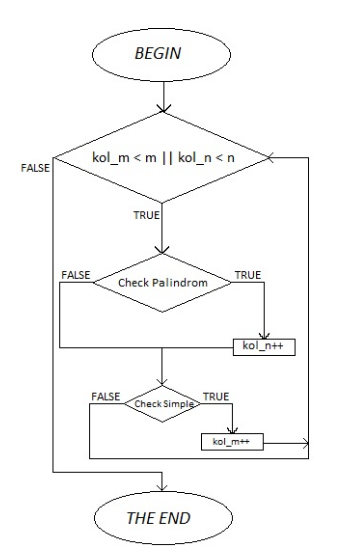
\includegraphics[width=0.5\textwidth]{block1.png}
\subsection{Результат}
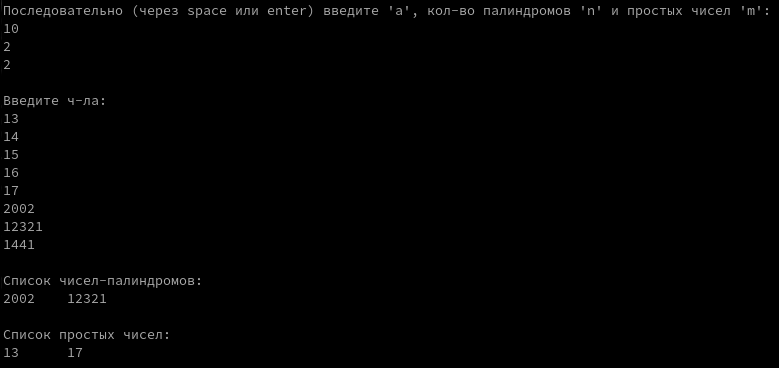
\includegraphics[width=1\textwidth]{1.png}
\newpage
\section{Задание №2} 
\subsection{Условие}
Вводится последовательность целых чисел, которая заканчивается после ввода n простых чисел. Для каждого введённого числа вывести его наибольший делитель, меньший самого числа.
\subsection{Код}
\small
\begin{verbatim}
#include <iostream>
using namespace std;
bool Check_Simple(int ch){
    int kol = 0;
    for (int i = 1; i <=ch; i++) if(ch % i == 0) kol++;
    if(kol == 2) return true;
    else return false;
}
int Del(int ch){
    int del = 0;
    for(int i = 1; i < ch; i++) if(ch % i == 0) del = i;
    return del;
}
int main(){
    int ch, n, kol_n = 0;
    cout << "Введите требуемое кол-во простых чисел n:  ";
    cin >> n;
    cout << "\nВведите числo:\n";
    cin >> ch;
    if(Check_Simple(ch)) kol_n++;
    cout << "наибольший делитель " << ch << ":  " << Del(ch) << endl;
    while(kol_n < n){
        cout << "\nВведите следующее число:\n";
        cin >> ch;
        if(Check_Simple(ch))kol_n++;
        cout << "наибольший делитель " << ch << ":  " << Del(ch) << endl;
    }
    return 0;
}
\end{verbatim}\normalsize
\subsection{Блок-схема}
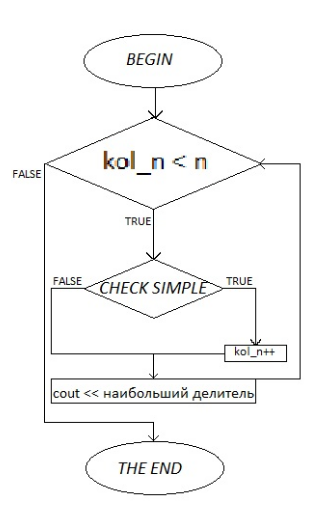
\includegraphics[width=0.7\textwidth]{block2.png}
\subsection{Результат}
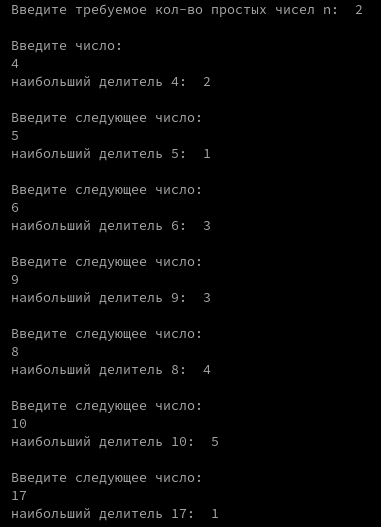
\includegraphics[width=0.9\textwidth]{2.png}
\newpage
\section{Задание №3} 
\subsection{Условие}
Найти сумму квадратов первых n (100\leq{n}\leq1000$)   чисел, кратных 7.
\subsection{Код}
\footnotesize
\begin{verbatim}
#include <iostream>
using namespace std;
int main(){
    int n, sum = 0;
    cout << "\n\tВведите кол-во чисел n:  "; cin >> n;
    cout << "\t";
    for(int i = 1; i <= n; i++)
        if(i % 7 == 0){
            cout << i << " "; 
            sum += i*i;
        }
    cout << "\n\tПолученная сумма из первых " << n << " чисел:  " << sum << endl << endl;
}
\end{verbatim}\normalsize
\subsection{Блок-схема}
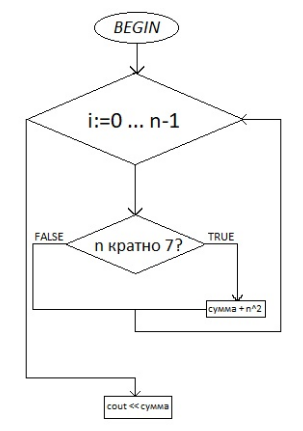
\includegraphics[width=0.9\textwidth]{block3.png}
\subsection{Результат}
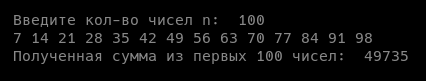
\includegraphics[width=1\textwidth]{3.png}
\subsection{Результат проверки в Wolfram}
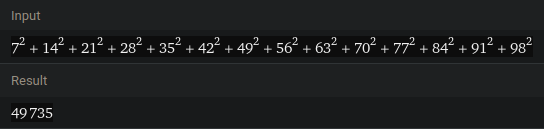
\includegraphics[width=1\textwidth]{wa1.png}
\newpage
\section{Задание №4} 
\subsection{Условие}
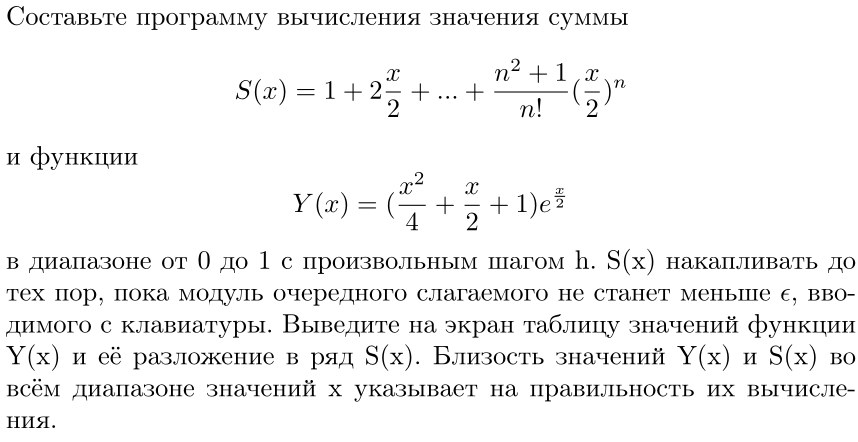
\includegraphics[width=1\textwidth]{task4.png}
\subsection{Код}
\small
\begin{verbatim}
#include <iostream>
#include <cmath>
using namespace std;
int Fact(int n){
    int pr = 1;
    while(n > 0){
        pr *= n;
        n-=1;
    }
    return pr;
}
int main(){
    float h, y, e;
    int n;
    cout << "h:  "; cin >> h;
    cout << "e:  "; cin >> e;
    for(float x = 0; x <= 1; x+=h){
        cout << "\nx: " << x;
        float s = 0;
        n = 0;
        while(fabs(((pow(n,2)+1)/Fact(n))*pow(x/2, n)) >= e){
            s += ((pow(n,2)+1)/Fact(n))*pow(x/2, n);
            n++;
        }
        y = (pow(x,2)/4 + x/2 + 1)*exp(x/2);
        cout << "\ts: " << s << "\ty: " << y;
    }
    return 0;
}
\end{verbatim}\normalsize
\subsection{Блок-схема}
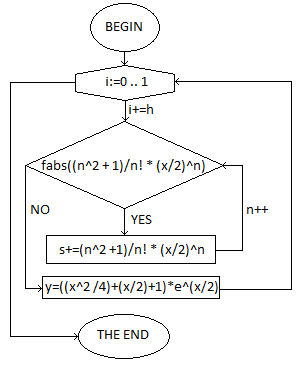
\includegraphics[width=0.7\textwidth]{block4.png}
\subsection{Результат}
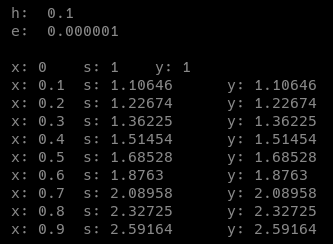
\includegraphics[width=1\textwidth]{4.png}
\newpage
\section{Задание №5} 
\subsection{Условие}
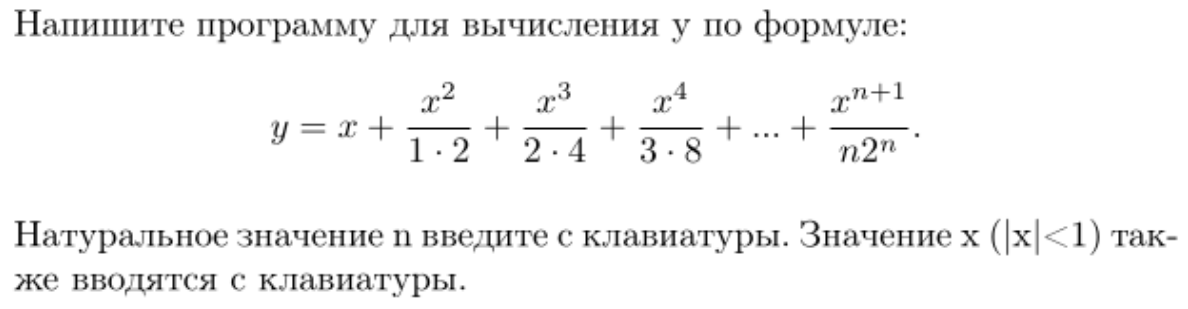
\includegraphics[width=1\textwidth]{task5.png}
\subsection{Код}
\small
\begin{verbatim}
#include <iostream>
#include <cmath>
using namespace std;
int main(){
    int n, x;
    float y = 0;
    cout << "Введите:\n";
    cout << "n:  "; cin >> n;
    cout << "x:  "; cin >> x;
    y+=x;
    for(int i = 1; i <= n; i++) y+=float(pow(x, i+1)/(i*pow(2, i)));
    cout << "y:  " << y << endl;
    return 0;
}
\end{verbatim}\normalsize
\subsection{Блок-схема}
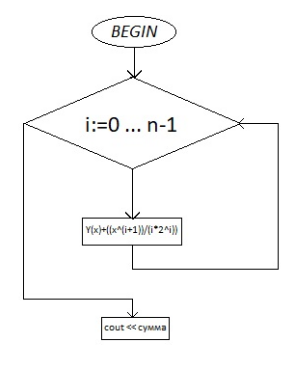
\includegraphics[width=1\textwidth]{block5.png}
\subsection{Результат}
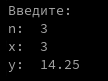
\includegraphics[width=1\textwidth]{5.png}
\subsection{Результат проверки в Wolfram}
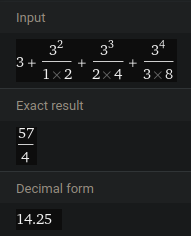
\includegraphics[width=1\textwidth]{wa2.png}
\end{document}
